\chapter{XPS of QA on the Ag(100) surface}
\label{chap:XPS}

\subsection{C1s XPS spectra}

\begin{figure}[H]
    \centering
    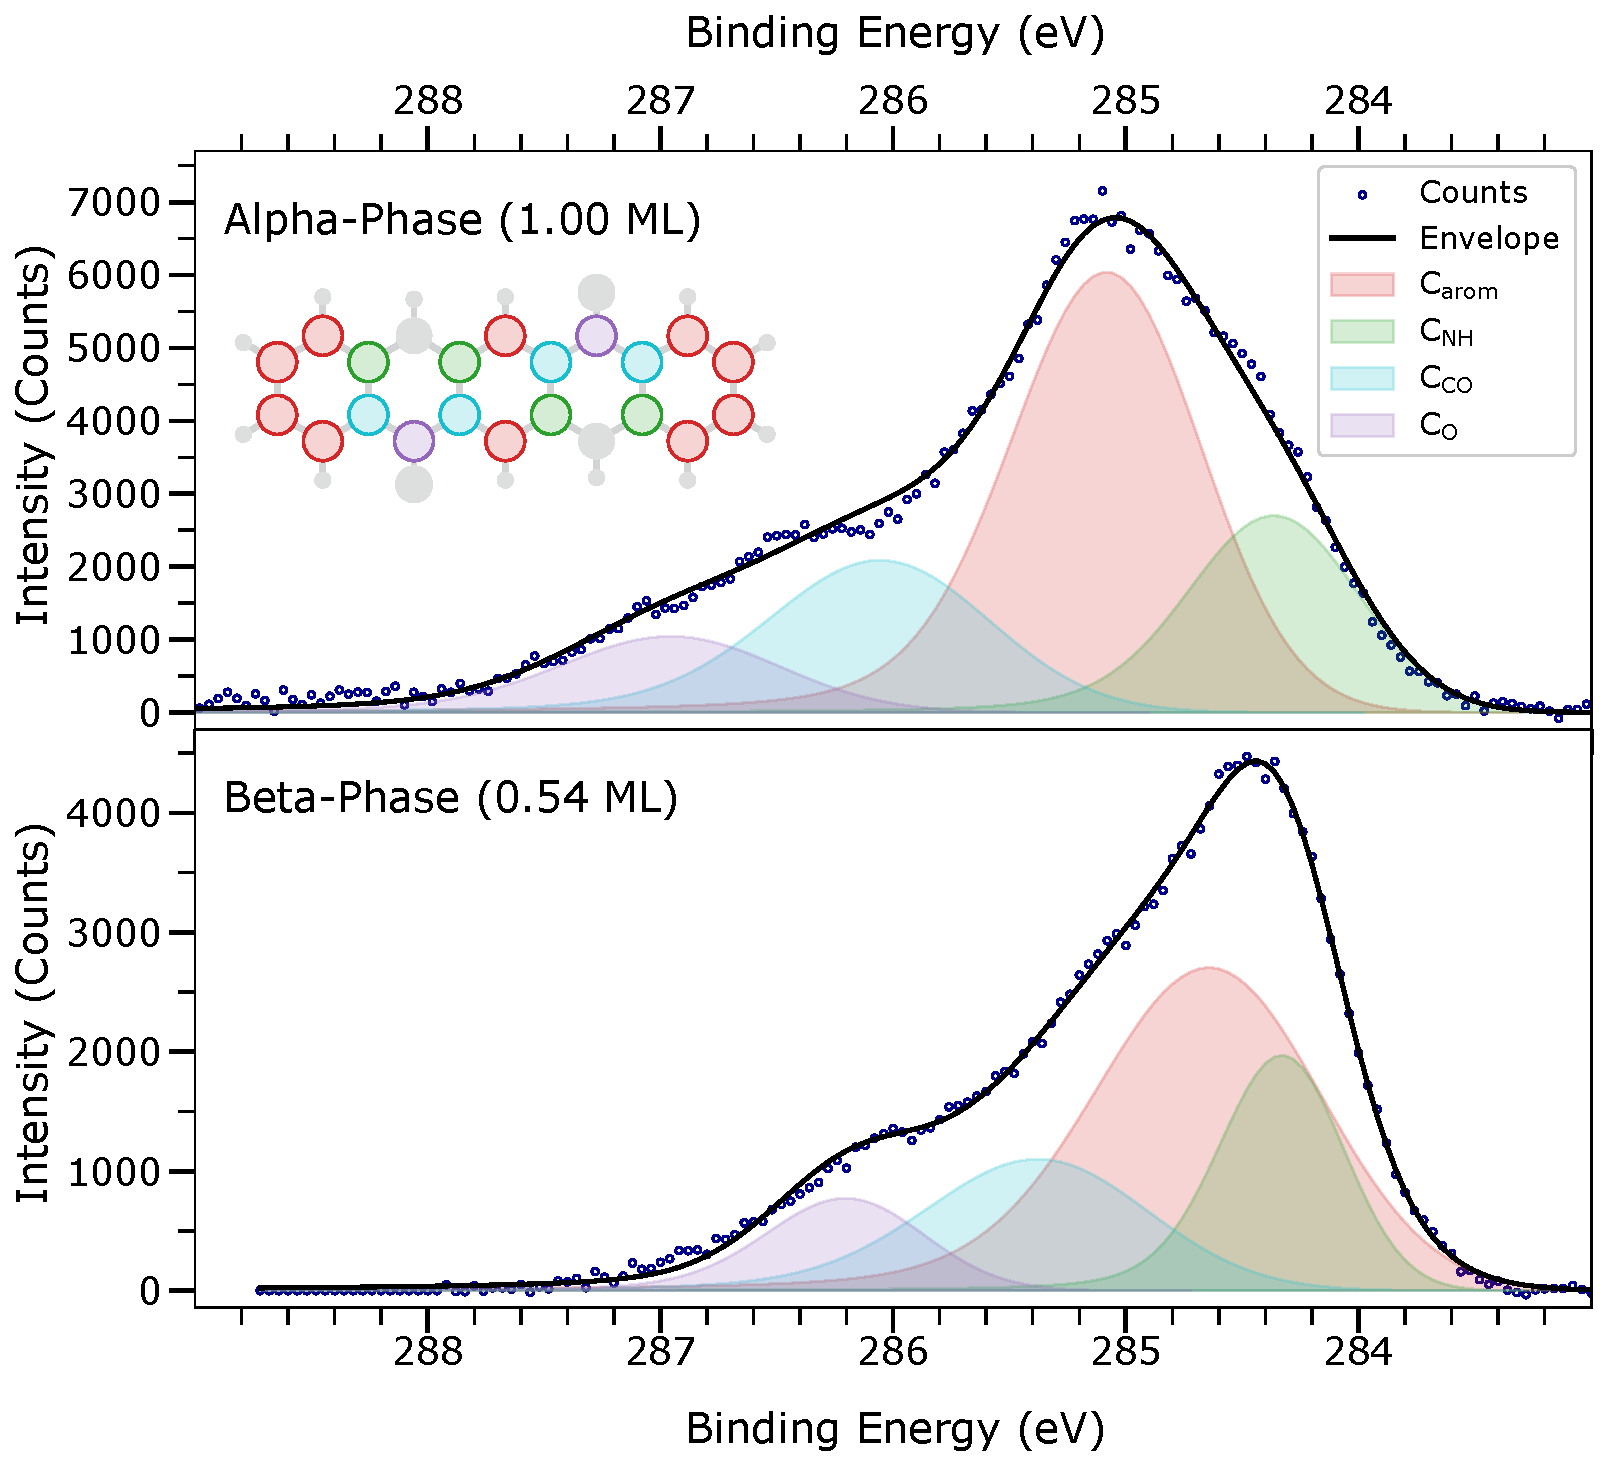
\includegraphics[width=\textwidth]{images/XPS-C1s.pdf}
    \caption{C1s \ac{XPS} spectra of \ac{QA} on the Ag(100) surface in the $\alpha$-phase and in the $\beta$-phase. The different fitted peaks are shown in different colors.}
    \label{fig:XPS-C1s-alpha}
\end{figure}

\begin{table}[H]
	\centering
	\caption{}
	\begin{tabular}{@{}ccccc@{}} \toprule
		 & peak & \ac{BE} / eV & FWHM / eV & area ratio \\
		\midrule
		$\alpha$-phase & $\mathrm{C_{arom}}$ & 285.00 & 0.95 & 10 \\
		& $\mathrm{C_{NH}}$ & 284.29 & 0.85 & 4 \\
		& $\mathrm{C_{CO}}$ & 285.96 & 1.1 & 4 \\ 
		& $\mathrm{C_{O}}$ & 286.86 & 1.1 & 2 \\
        \midrule
		$\beta$-phase & $\mathrm{C_{arom}}$ & 284.54 & 1.13 & 10 \\
		& $\mathrm{C_{NH}}$ & 284.27 & 0.62 & 4 \\
		& $\mathrm{C_{CO}}$ & 285.28 & 1.11 & 4 \\ 
		& $\mathrm{C_{O}}$ & 285.13 & 0.79 & 2 \\
		\bottomrule
	\end{tabular}
	\label{tab:XPS-C1s-fit}
\end{table}

\begin{figure}[H]
    \centering
    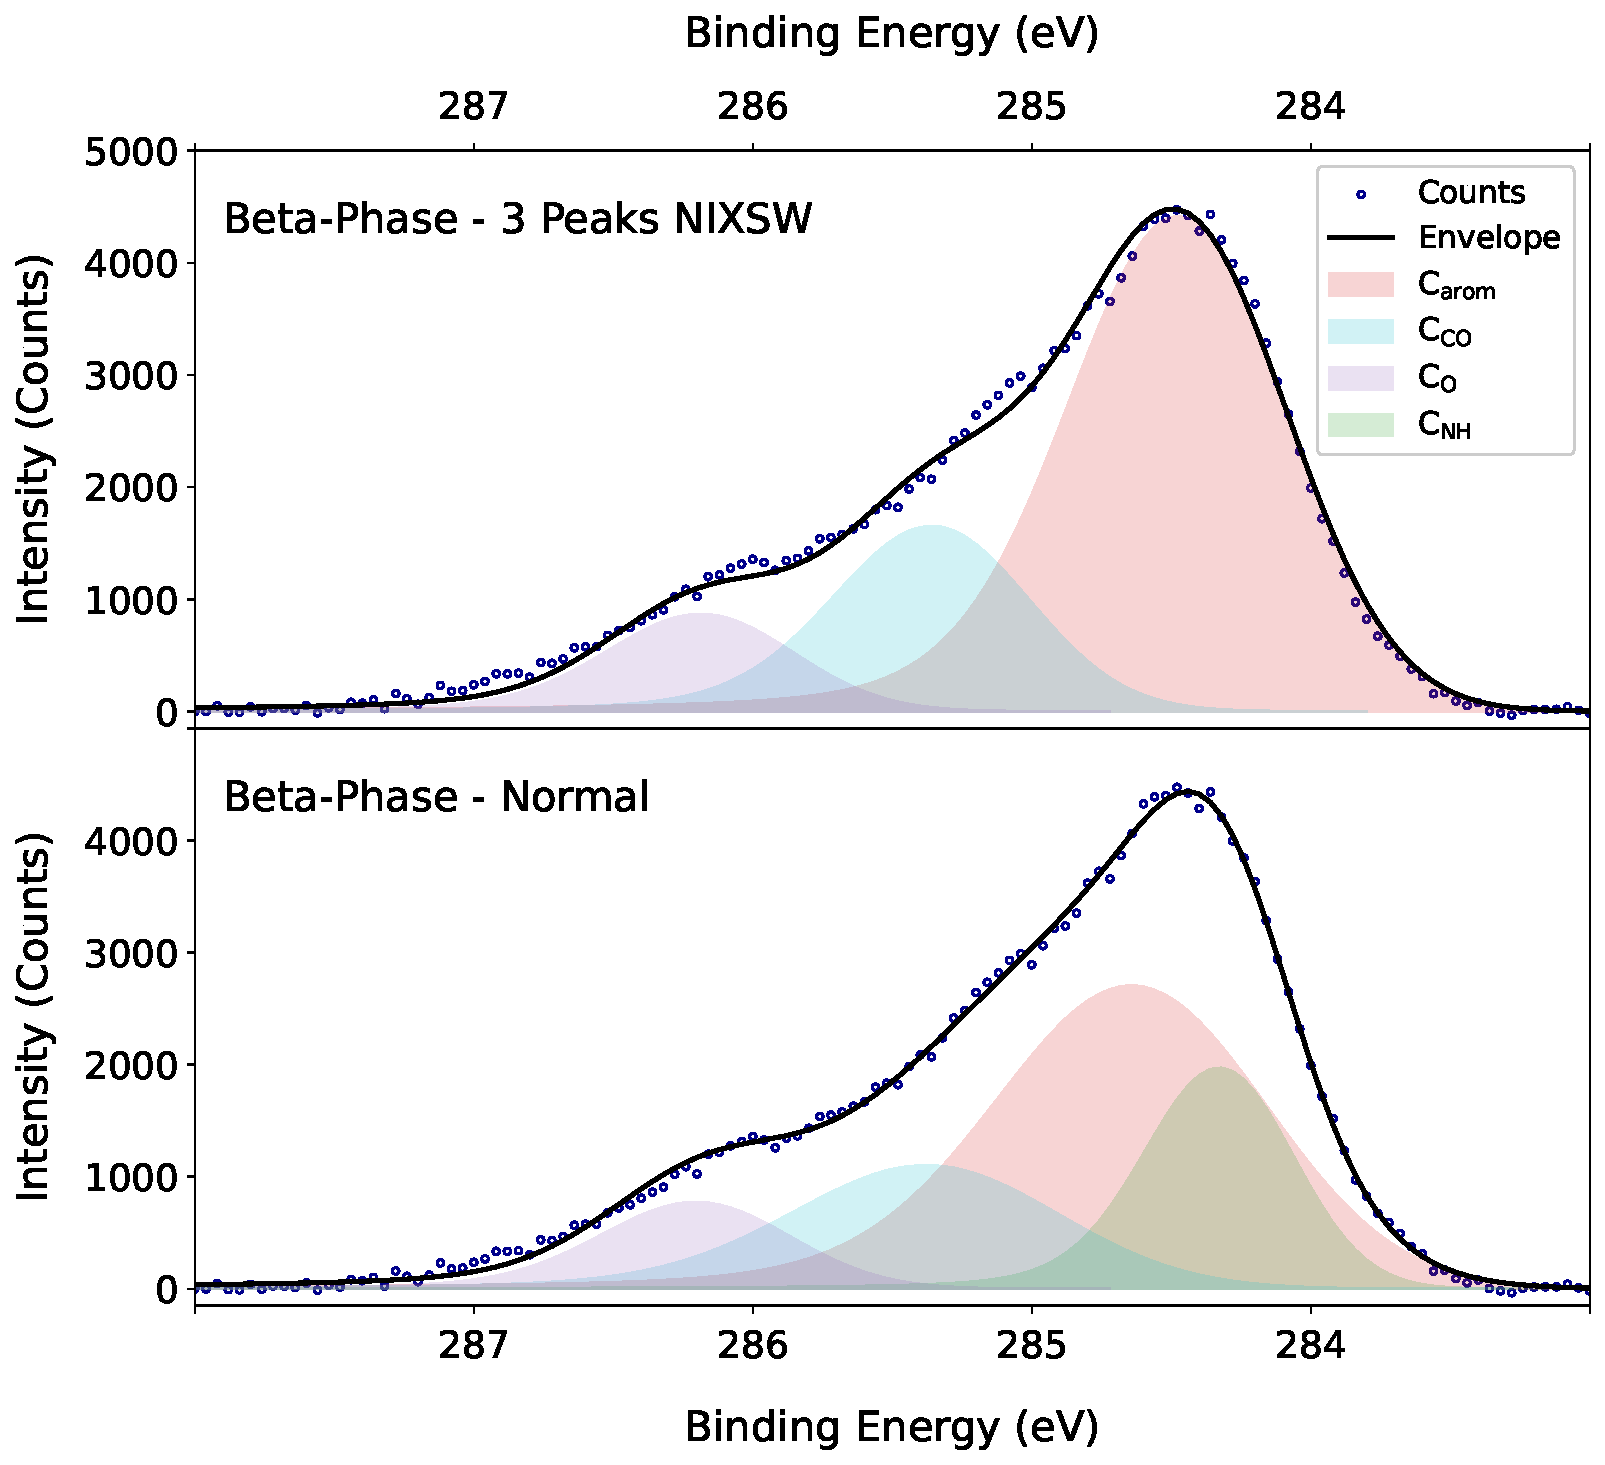
\includegraphics[width=\textwidth]{images/XPS-C1s-3Peaks.pdf}
    \caption{C1s \ac{XPS} spectra of \ac{QA} on the Ag(100) surface in the $\beta$-phase. The different fitted peaks are shown in different colors.}
    \label{fig:XPS-C1s-3peaks}
\end{figure}

\begin{table}[H]
	\centering
	\caption{}
	\begin{tabular}{@{}ccccc@{}} \toprule
		 & peak & \ac{BE} / eV & area ratio & FWHM / eV \\
		\midrule
		$\beta$-phase - 4 peaks & $\mathrm{C_{arom}}$ & 284.54 & 1.13 & 10 \\
		& $\mathrm{C_{NH}}$ & 284.27 & 0.62 & 4 \\
		& $\mathrm{C_{CO}}$ & 285.28 & 1.11 & 4 \\ 
		& $\mathrm{C_{O}}$ & 285.13 & 0.79 & 2 \\
        \midrule
		$\beta$-phase - 3 peaks & $\mathrm{C_{arom}}+\mathrm{C_{NH}}$ & 284.39 & 0.92 & 14 \\
		& $\mathrm{C_{CO}}$ & 285.29 & 0.82 & 4 \\ 
		& $\mathrm{C_{O}}$ & 286.12 & 0.78 & 2 \\
		\bottomrule
	\end{tabular}
	\label{tab:XPS-C1s-fit-3peaks}
\end{table}

\newpage
\subsection{O1s XPS spectra}

\begin{figure}[H]
    \centering
    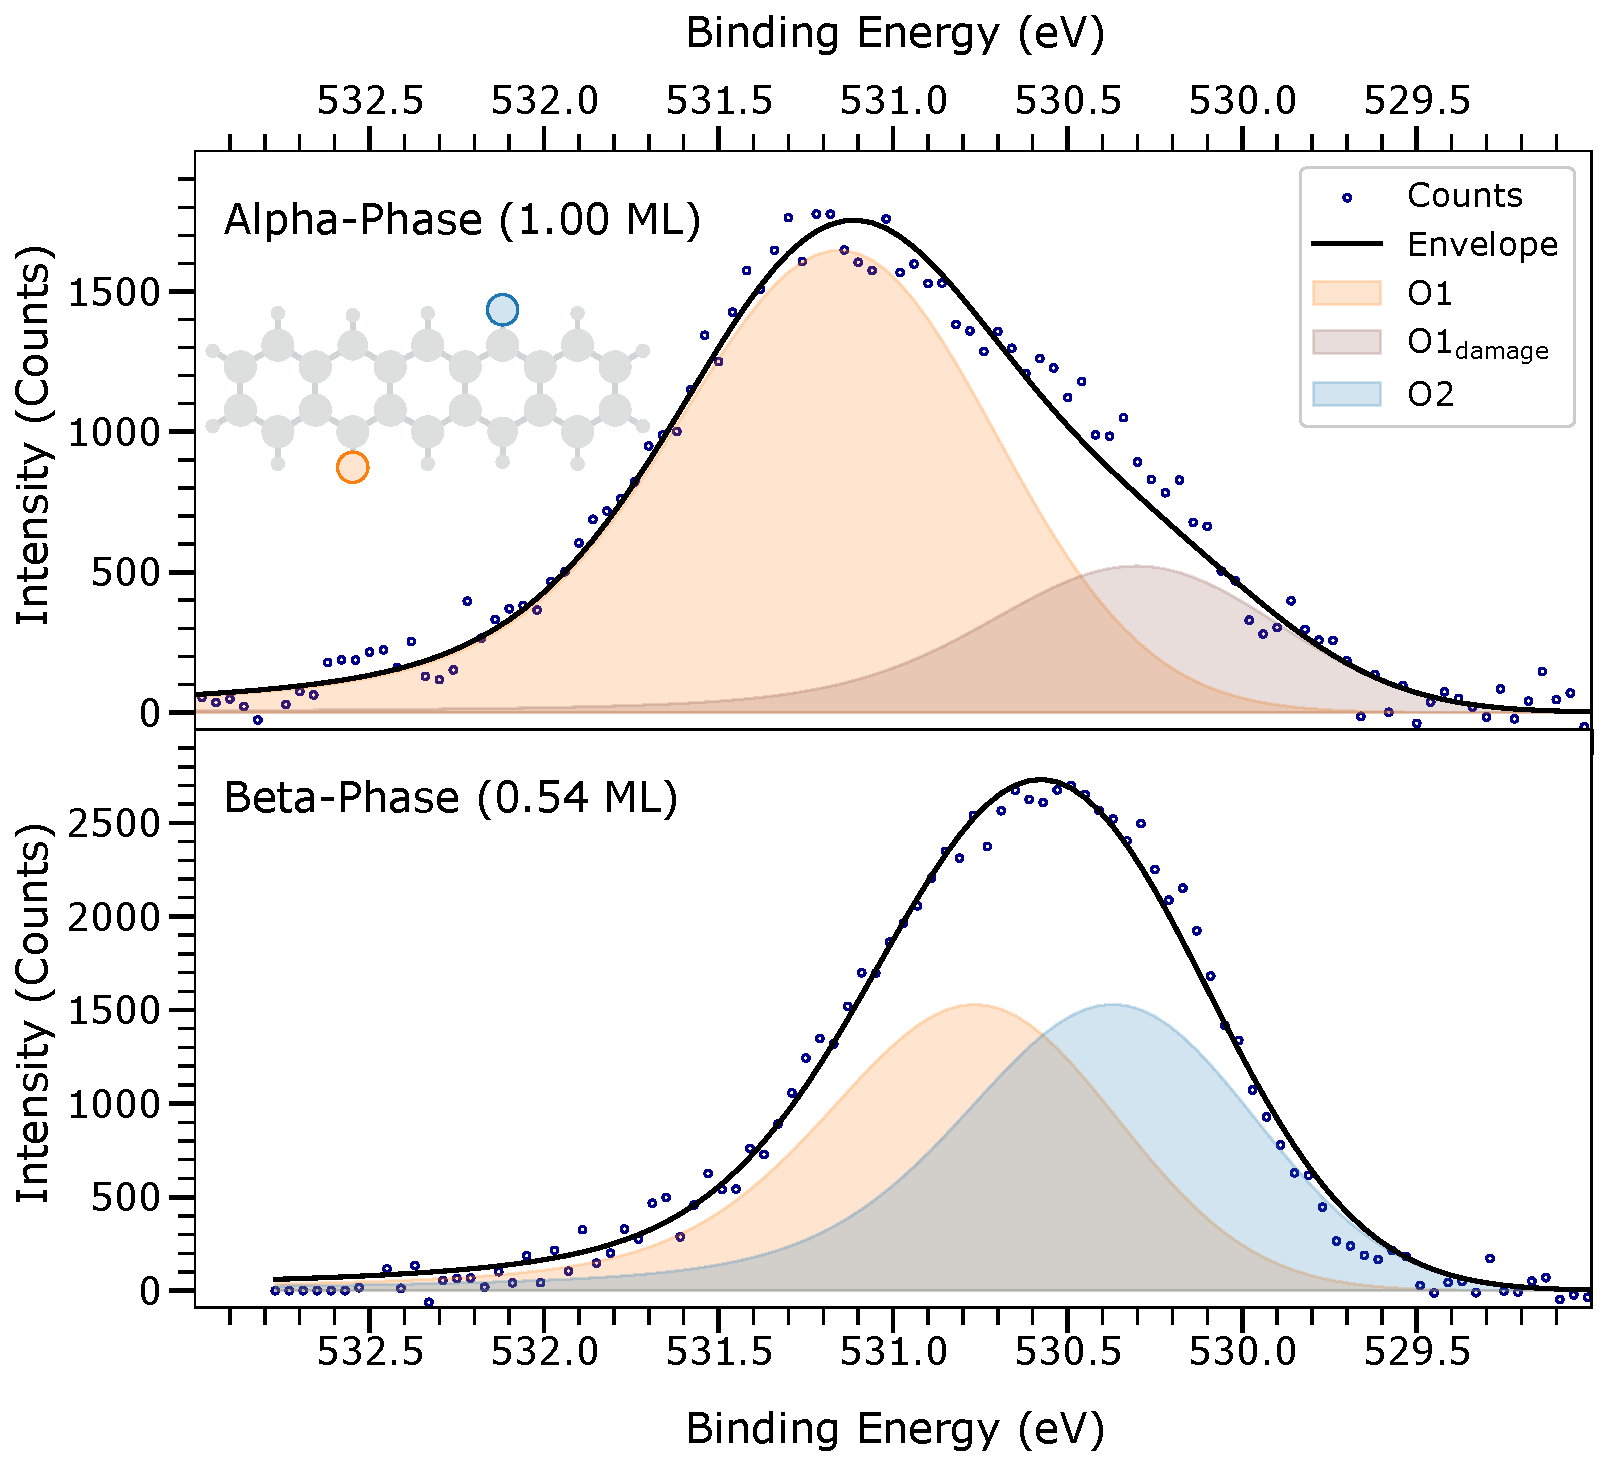
\includegraphics[width=\textwidth]{images/XPS-O1s.pdf}
    \caption{O1s \ac{XPS} spectra of \ac{QA} on the Ag(100) surface in the $\alpha$-phase and in the $\beta$-phase. The different fitted peaks are shown in different colors.}
    \label{fig:XPS-O1s-alpha}
\end{figure}

\begin{table}[H]
	\centering
	\caption{}
	\begin{tabular}{@{}ccccc@{}} \toprule
		 & peak & \ac{BE} / eV & FWHM / eV & area ratio \\
		\midrule
		$\alpha$-phase & $\mathrm{O1}$ & 531.02 & 1.05 & 1 \\
		& $\mathrm{O1_{damage}}$ & 530.18 & 0.95 & - \\
        \midrule
		$\beta$-phase & $\mathrm{O1}$ & 530.64 & 0.95 & 1 \\
		& $\mathrm{O2}$ & 530.25 & 0.95 & 1 \\
		\bottomrule
	\end{tabular}
	\label{tab:XPS-O1s-fit}
\end{table}

\newpage
\subsection{N1s XPS spectra}

\begin{figure}[H]
    \centering
    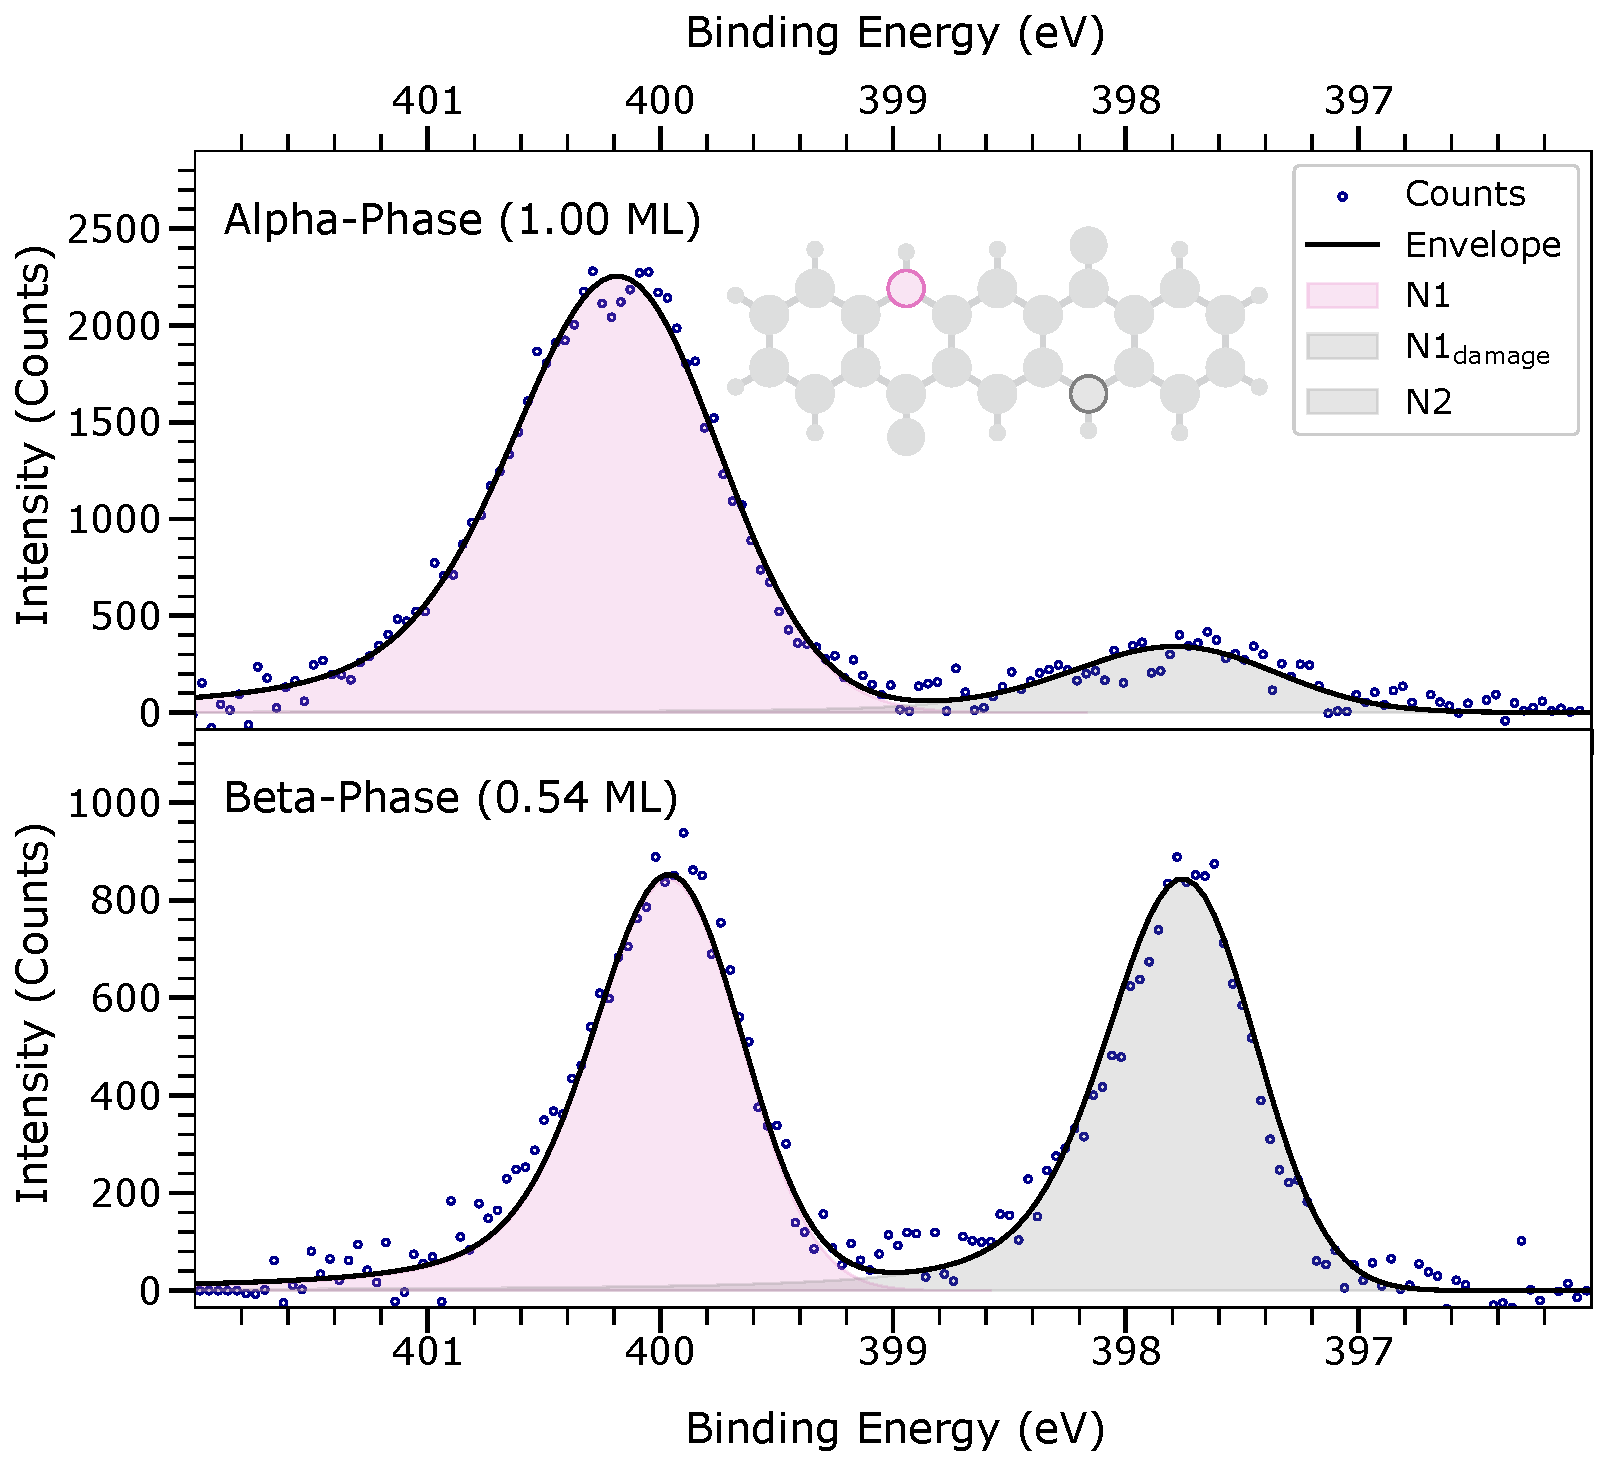
\includegraphics[width=\textwidth]{images/XPS-N1s.pdf}
    \caption{N1s \ac{XPS} spectra of \ac{QA} on the Ag(100) surface in the $\alpha$-phase and in the $\beta$-phase. The different fitted peaks are shown in different colors.}
    \label{fig:XPS-N1s-alpha}
\end{figure}

\begin{table}[H]
	\centering
	\caption{}
	\begin{tabular}{@{}ccccc@{}} \toprule
		 & peak & \ac{BE} / eV & FWHM / eV & area ratio \\
		\midrule
		$\alpha$-phase & $\mathrm{N1}$ & 400.05 & 1.02 & 1 \\
		& $\mathrm{N1_{damage}}$ & 397.66 & 1.02 & - \\
        \midrule
		$\beta$-phase & $\mathrm{N1}$ & 399.87 & 0.73 & 1 \\
		& $\mathrm{N2}$ & 397.66 & 0.73 & 1 \\
		\bottomrule
	\end{tabular}
	\label{tab:XPS-N1s-fit}
\end{table}

%%%%%%%%%%%%%%%%%%%%%%%%%%%%%%%%%%%%%%%%%%%%%%%%%%%%%%%%%%%%%%%%%%%%%%%%%%%%%%%%%%%%%%%

\cleardoublepage
\chapter{NIXSW of QA on the Ag(100) surface}

\section{The \texorpdfstring{$\alpha$}{alpha}-phase}

\subsection{C1s NIXSW spectra}

\begin{figure}
    \centering
    
\includegraphics[width=0.8\textwidth]{images/NIXSW_C1s_Alpha.pdf}
    \caption{C1s \ac{NIXSW} spectra of \ac{QA} on the Ag(100) surface in the $\alpha$-phase. The different fitted peaks are shown in different colors.}
    \label{fig:NIXSW-C1s-alpha}
\end{figure}

\begin{table}[H]
	\centering
	\caption{}
	\begin{tabular}{@{}cccc@{}} \toprule
		 & $f_c$ & $p_c$ & d (\si{\angstrom}) \\
		\midrule
		$\mathrm{C_{arom}}$ &  &  &  \\
		$\mathrm{C_{NH}}$ &  &  &  \\
		$\mathrm{C_{CO}}$ &  &  &  \\ 
		$\mathrm{C_{O}}$ &  &  &  \\
        $\mathrm{C_{total}}$ & & & \\
		\bottomrule
	\end{tabular}
	\label{tab:NIXSW-C1s-alpha}
\end{table}

\newpage
\subsection{O1s NIXSW spectra}

\begin{figure}[H]
    \centering
    
\includegraphics[width=0.8\textwidth]{images/NIXSW_O1s_Alpha.pdf}
    \caption{O1s \ac{NIXSW} spectra of \ac{QA} on the Ag(100) surface in the $\alpha$-phase. The different fitted peaks are shown in different colors.}
    \label{fig:NIXSW-O1s-alpha}
\end{figure}

\begin{table}[H]
	\centering
	\caption{}
	\begin{tabular}{@{}cccc@{}} \toprule
		 & $f_c$ & $p_c$ & d (\si{\angstrom}) \\
		\midrule
		$\mathrm{O1}$ &  &  &  \\
		$\mathrm{O1_{damage}}$ &  &  &  \\ 
        $\mathrm{O_{total}}$ & & & \\
		\bottomrule
	\end{tabular}
	\label{tab:NIXSW-O1s-alpha}
\end{table}

\newpage 
\subsection{N1s NIXSW spectra}

\begin{figure}[H]
    \centering
    
\includegraphics[width=0.8\textwidth]{images/NIXSW_N1s_Alpha.pdf}
    \caption{N1s \ac{NIXSW} spectra of \ac{QA} on the Ag(100) surface in the $\alpha$-phase. The different fitted peaks are shown in different colors.}
    \label{fig:NIXSW-N1s-alpha}
\end{figure}

\begin{table}[H]
	\centering
	\caption{}
	\begin{tabular}{@{}cccc@{}} \toprule
		 & $f_c$ & $p_c$ & d (\si{\angstrom}) \\
		\midrule
		$\mathrm{N1}$ &  &  &  \\
		$\mathrm{N1_{damage}}$ &  &  &  \\ 
        $\mathrm{N_{total}}$ & & & \\
		\bottomrule
	\end{tabular}
	\label{tab:NIXSW-N1s-alpha}
\end{table}

%%%%%%%%%%%%%%%%%%%%%%%%%%%%

\newpage
\section{The \texorpdfstring{$\beta$}{beta}-phase}

\subsection{C1s NIXSW spectra}

\begin{figure}[H]
    \centering
    
\includegraphics[width=0.8\textwidth]{images/NIXSW_C1s_Beta.pdf}
    \caption{C1s \ac{NIXSW} spectra of \ac{QA} on the Ag(100) surface in the $\beta$-phase. The different fitted peaks are shown in different colors.}
    \label{fig:NIXSW-C1s-beta}
\end{figure}

\begin{table}[H]
	\centering
	\caption{}
	\begin{tabular}{@{}cccc@{}} \toprule
		 & $f_c$ & $p_c$ & d (\si{\angstrom}) \\
		\midrule
		$\mathrm{C_{arom}}+\mathrm{C_{NH}}$ &  &  &  \\
		$\mathrm{C_{CO}}$ &  &  &  \\ 
		$\mathrm{C_{O}}$ &  &  &  \\
        $\mathrm{C_{total}}$ & & & \\
		\bottomrule
	\end{tabular}
	\label{tab:NIXSW-C1s-beta}
\end{table}

\newpage
\subsection{O1s NIXSW spectra}

\begin{figure}[H]
    \centering
    
\includegraphics[width=0.8\textwidth]{images/NIXSW_O1s_Beta.pdf}
    \caption{O1s \ac{NIXSW} spectra of \ac{QA} on the Ag(100) surface in the $\beta$-phase. The different fitted peaks are shown in different colors.}
    \label{fig:NIXSW-O1s-beta}
\end{figure}

\begin{table}[H]
	\centering
	\caption{}
	\begin{tabular}{@{}cccc@{}} \toprule
		 & $f_c$ & $p_c$ & d (\si{\angstrom}) \\
		\midrule
		$\mathrm{O1}$ &  &  &  \\
		$\mathrm{O2}$ &  &  &  \\ 
        $\mathrm{O_{total}}$ & & & \\
		\bottomrule
	\end{tabular}
	\label{tab:NIXSW-O1s-beta}
\end{table}

\newpage
\subsection{N1s NIXSW spectra}

\begin{figure}[H]
    \centering
    
\includegraphics[width=0.8\textwidth]{images/NIXSW_N1s_Beta.pdf}
    \caption{N1s \ac{NIXSW} spectra of \ac{QA} on the Ag(100) surface in the $\beta$-phase. The different fitted peaks are shown in different colors.}
    \label{fig:NIXSW-N1s-beta}
\end{figure}

\begin{table}[H]
	\centering
	\caption{}
	\begin{tabular}{@{}cccc@{}} \toprule
		 & $f_c$ & $p_c$ & d (\si{\angstrom}) \\
		\midrule
		$\mathrm{N1}$ &  &  &  \\
		$\mathrm{N2}$ &  &  &  \\ 
        $\mathrm{N_{total}}$ & & & \\
		\bottomrule
	\end{tabular}
	\label{tab:NIXSW-N1s-beta}
\end{table}

\newpage
\subsubsection{Overview of the \texorpdfstring{$\alpha$}{alpha}- and \texorpdfstring{$\beta$}{beta}-phase}

\begin{figure}[H]
    \centering
    \begin{subfigure}[b]{0.48\textwidth}
        \centering
        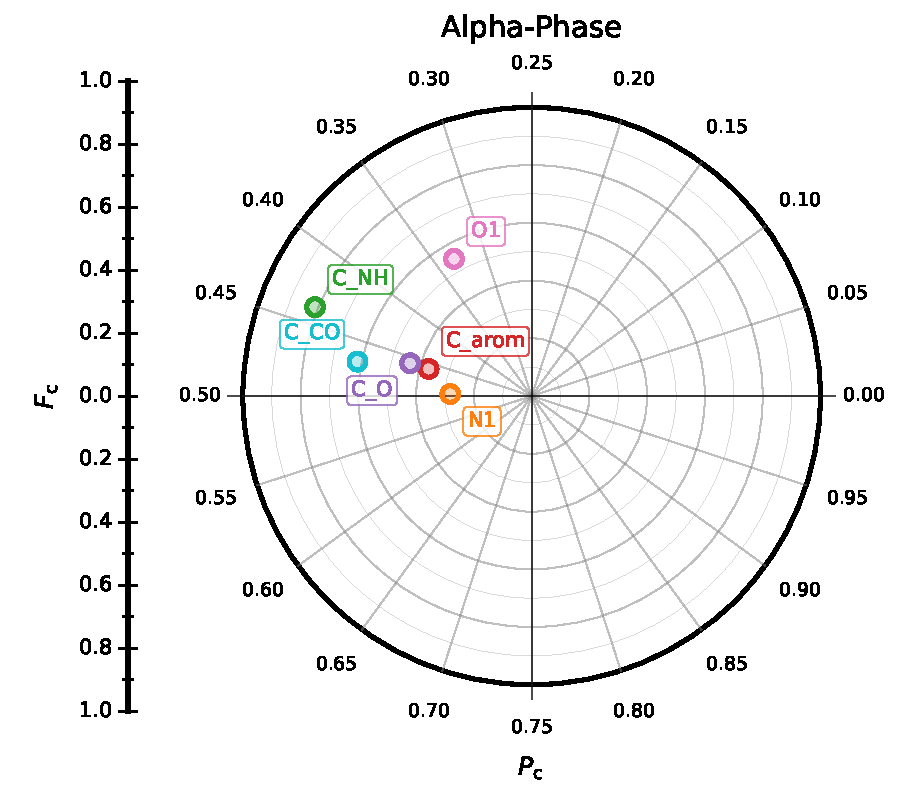
\includegraphics[width=\linewidth]{images/Argand_Alpha.pdf}
        \caption{$\alpha$-phase}
        \label{fig:Argand-alpha}
    \end{subfigure}\hfill
    \begin{subfigure}[b]{0.48\textwidth}
        \centering
        
\includegraphics[width=\linewidth]{images/Argand_Beta.pdf}
        \caption{$\beta$-phase}
        \label{fig:Argand-beta}
    \end{subfigure}
    \caption{Overview of the Argand representations for the $\alpha$- and $\beta$-phases.}
    \label{fig:Argand-overview}
\end{figure}

\cleardoublepage